\section{Introducción y configuraciones circuitales}

En el presente informe se realizará un análisis teórico y experimental del comportamiento y características de las configuraciones 
circuitales planteadas empleando un amplificador operacional del integrado LM324. 

Con cada circuito, se iniciará con un estudio de distintos modelos teóricos para entender su respuesta en frecuencia y su impedancia de entrada; seguidamente
se hará hincapié en las propiedades, limitaciones y efectos sobre la tensión de entrada inyectada en el operacional junto; se finalizára el informe con el estudio de la 
respuesta del operacional bajo determinadas condiciones. 

A lo largo del trabajo, se dejará constancia de los inconvenientes y problemas que se tuvieron durante la realización de las mediciones sobre los circuitos con el fin de recibir una devolución con
la correción e incorporarlas en las próximas instancias.

En este informe se analizarán características y comportamientos de los siguientes circuitos:

\begin{figure}[H]
	\centering
	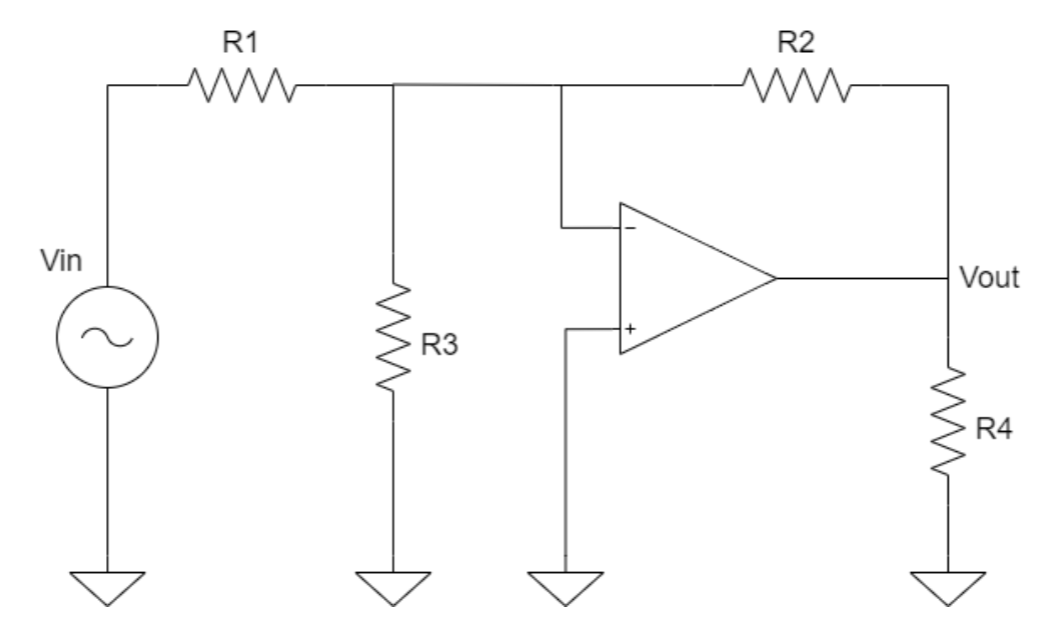
\includegraphics[scale=0.3]{./Imagenes/circInversor.png}
	\caption{Circuito inversor}
	\label{fig:circInv}
\end{figure}

\begin{figure}[H]
	\centering
	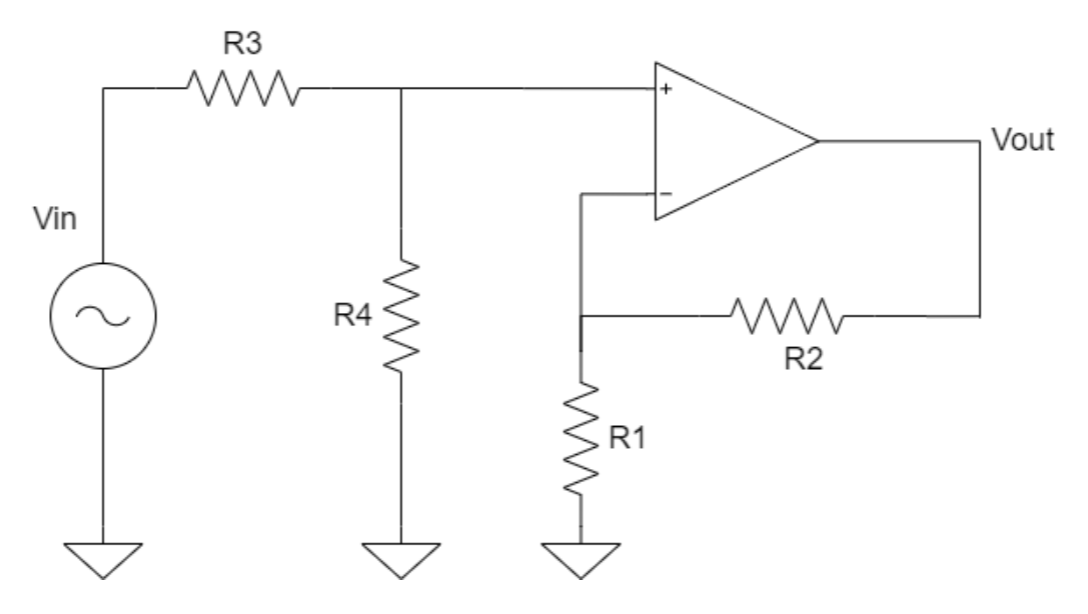
\includegraphics[scale=0.3]{./Imagenes/circNoInversor.png}
	\caption{Circuito no inversor}
	\label{fig:circNoInv}
\end{figure}

Considerando los siguientes casos:

\begin{table}[H]
\centering
\begin{tabular}{c|ccc}
       & $R_{1}=R_{3}$ &   $R_{2}$   & $R_{4}$   \\ \hline
Caso 1 & $2.7k\Omega$  & $27k\Omega$  & $10k\Omega$  \\
Caso 2 & $2.7k\Omega$  & $2.7k\Omega$ & $10k\Omega$  \\
Caso 3 & $27k\Omega$   & $2.7k\Omega$ & $100k\Omega$
\end{tabular}
\end{table}
